\documentclass[twocolumn]{aastex62}

\newcommand{\vdag}{(v)^\dagger}
\newcommand\aastex{AAS\TeX}
\newcommand\latex{La\TeX}
\usepackage{amsmath}
\usepackage{physics}
\usepackage{hyperref}
\usepackage{natbib}
\usepackage[T1]{fontenc}
\usepackage[english]{babel}
\usepackage[utf8]{inputenc}
\usepackage{wasysym}

\begin{document}

\title{\Large AST5220-Milestone IV: The CMB and Matter Power-Spectra}

\author{Nils-Ole Stutzer}

\begin{abstract}
    
    \textit{The codes for this paper can be found at:} \newline \url{https://github.com/SagittariusA-Star/AST5220-Milestones}
\end{abstract}

\section{Introduction} \label{sec:Intro}
The aim of cosmology as a science has always been to unearth the secretes of how the Universe was formed and how it has evolved since. As modern high precision
measurements by probes like Planck have shown is how successful the cosmological standard model with dark energy and cold dark matter ($\Lambda$CDM) is in describing the observed data of the CMB and its anisotropies \citep[]{planckcollaboration:2018}. One of the most common ways to estimate the parameter values of the $\Lambda$CDM model infered from the data, is to compare the observed and the theoretical CMB and matter power spectra and find the best-fit by means of a statistical treatment. 

In this paper we will focus on computing the CMB and matter power spectra, by building upon the foundation by \cite{stutzer:2020a}, \cite{stutzer:2020b} and \cite{stutzer:2020c} which computed the background evolution, recombination history and formation of structure from primordial perturbations of the Universe. The ultimate goal of computing the power spectra will be achieved using the same cosmological parameters as \cite{callin:2006}, also previously used in \cite{stutzer:2020a}, \cite{stutzer:2020b} and \cite{stutzer:2020c}. Further more, we will for simplicity neglect the spatial curvature, neutrinos and polarization of photons. 


\section{Method} \label{sec:Method}
When solving for the CMB and matter power spectra in this paper we will mainly use the equations and relations that are provided by \cite{winther:2020c}, \cite{callin:2006} and \cite{dodelson:2003}. Unless otherwise stated the equations presented here are thus provided by these authors and refere the interested reader to them for detailed derivations, and only present the main outline towards computing the power spectra.  


\subsection{The Power Spectra} \label{subsec:spectra}
Before going on to actually computing the power spectra, a few words on what a power spectrum actually is. To find out this we consider the CMB as an example. The CMB as we see it today is build up of an average temperature of $T_\mathrm{CMB} = 2.7255\mathrm{K}$ upon which there are small perturbations of the order $\delta T / T_\mathrm{CMB} \sim 10^{-5}$ seen as anisotropies in the CMB. One can think of the CMB of a function on the celestial sphere that can be expanded in term of its anisotropies of different scales as basis functions. This is done using spherical harmonics as 
\begin{align}
    T(\hat{n}) = \sum_{\ell m} a_{\ell m} Y_{\ell m}(\hat{n}),
\end{align}
where the temperature $T$ in the direction $\hat{n}$ on the sky is given by the sum over the spherical harmonics $Y_{\ell m}$ times the corresponding expansion coefficient $a_{\ell m}$. The indices $\ell$ and $m$ quantify the scale and orientation of the perturbations. For instance $\ell = 0$, $\ell = 1$ and $\ell = 2$ represent the monopole (average temperature), dipole (hot and cold blobs separated by $180^\circ$ on the sky) and the quadrupole (alternating hot and cold separated by $90^\circ$ on the sky).

The angular power spectrum of the CMB anisotropies is simply related to this expansion and corresponds to the expected value of the expansion coefficient squared for each scale $\ell$
\begin{align}
    C_\ell = \langle |a_{\ell m}|^2 \rangle = \langle a_{\ell m}a_{\ell m}^* \rangle.
\end{align}
In principle, though, there should be a dependence on the orientation $m$, however, since the CMB according to the underlying cosmological principle must be isotropic on large scales we can simply average out the directional dependence without large errors. The angular power spectrum $C_\ell$ hence quantifies how much contribution to the CMB there is on each angular scale, i.e. the amplitude, and can be understood as a correlation function between to points of a given angular separation. 

In order to compute the power spectrum $C_\ell$ we need the coefficients $a_{\ell m}$ which are given by the temperature field at time $x = \ln a(t)$ $T(\hat{n}, x)$. The temperature fields evolution through time $x$ and for different scales $k$ were found in \cite{stutzer:2020c} in the form of the photon perturbation multipole moments $\Theta_\ell(k, x)$. These multipole moments were however found in fourier $\vec{k}$-space, but we want to have them in real ($\vec{n}$-) space at the present time. To get the perturbations $\Theta_\ell(\hat{n}, x)$ today, we simply inverse fourier transform and evaluate the result at the present time $x = 0$. 

There is only one caveat to this idea. In order to compute all the coefficients $a_{\ell m}$ we would need the infinite series of multipole monents $\Theta_\ell$, however, \cite{stutzer:2020c} only computed around 8 of them, but we would need around $\ell_text{max} \sim 1200$ to get a decent power spectrum \citep[]{winther:2020c}. Solving for all the multipole moments up to $\ell = 1200$ using the approach of \cite{stutzer:2020c} would take a long time and be very inefficient. 

Fortunately Zaldarriaga and Seljak solved this problem for us by inventing the \textit{line-of-sight} integration. To obtain the coupled equations for the$ \Theta_\ell$'s in the first place one used the photon perturbation $\Theta(k, \mu, x)$, being a function of angle $\mu = \cos \theta$. Thus one can, instead expanding the perturbation equation into multipoles and then solving the long coupled system of differential equations as in \cite{stutzer:2020c} (but with $\ell_\text{max} = 1200$), integrate up the equation for the underlying $\dot{\Theta}$ subsequently find the multipoles. This is shown in detail by \cite{callin:2006} and \cite{dodelson:2003} and yields the following integral for the multipoles 
\begin{align}
    \Theta_\ell(k, x=0) = \int_{-\infty}^{0} \tilde{S}(k,x)
              j_\ell[k(\eta_0-\eta)] dx,
    \label{eq:transfer}
\end{align} 
where $j_ll$ are the spherical Bessel functions being highly oscillatory functions function as an orthogonal basis here that basically project the project the 3D spatial temperature field onto the 2D celestial sphere (as we observe it) and $\eta$ (subscript 0) is the conformal time (today). The $Theta_\ell(k, x = 0)$ is also called the transfer function and quantifies the multipole moments of the photons for each scale.

The quantity $\tilde{S}(k,x)$ is called the source function and is given by
\begin{align}
    \tilde{S}(x, k) &= \tilde{g}\left[ \Theta_0 + \Psi + \frac{1}{4}\Pi\right] + e^{-\tau} \left[\Psi^\prime-\Phi^\prime\right] \nonumber\\
    &- \frac{1}{ck}\frac{d}{dx}(\mathcal{H}\tilde{g}v_b) + \frac{3}{4c^2k^2} \frac{d}{dx} \left[\mathcal{H}\frac{d}{dx} (\mathcal{H}\tilde{g}\Pi)\right],
    \label{eq:source}
\end{align}
where the metric potential perturbations $\Psi$ and $\Phi$, the baryon velocity $v_b$ and the photon mono- and quadrupole $\Theta_0$ and $\Theta_2$ ($\Pi = \Theta_2$ if polarization is neglected) are all computed by \cite{stutzer:2020c}. The optical depth $\tau$ and visibility function $\tilde{g}$, and the reduced Hubble parameter $\mathcal{H}$ are found by \cite{stutzer:2020b} and \cite{stutzer:2020a} respectively. The source function quantifies how light is affected (both extinction and emission) when traveling through a medium, which in our case is the universe.

This approach of finding the multipoles $Theta_\ell$ is much faster as we only need $Theta_0$ and $\Theta_2$ from the coupled set of ODEs and it has the advantage of being easier to understand. Intuitively one can interpret the line-of-sight integration as integrating up a local radiation monopole through the universes history, which is represented by the term $\tilde{g}\Theta_0$. The terms $tilde{g}\Psi$ and $\tilde{g}\frac{1}{4}\Pi$ are corrections from the photons loosing energy through the potential wells and the correction of the local quadrupole (polarization if included) respectively. Secondly one can spot how the radiation field is affected by the change of the gravitational potentials, seen in the second part of $\tilde{S}$, and represents the gain in energy through the so-called Integrated Sachs-Wolf (ISW) effect. Basically the ISW is that photons that fall into a potential well will gain energy, but lose less than they gained when exiting, since the gravitational wells have decayed due to spatial expansion while the photon traveled through it. The third part of $\tilde{S}$ is simply a doppler effect term.

Now that we have all the $\Theta_\ell$'s we can finally find the power spectrum $C_\ell$. As computed by \cite{stutzer:2020c} the metric perturbations are initially of order $\Psi \sim 1$ which was the underlying initial condition for the whole set of coupled equations for the perturbations. To get the actual initially condition set up by inflation the multipoles (squared) are simply multiplied by the primordial power spectrum, given by the Harrison-Zel'dovich spectrum $P_\text{primordial}(k)$ given by
\begin{align}
    \frac{k^3}{2\pi^2} P_{\rm primordial}(k) = A_s \left(\frac{k}{k_{\rm pivot}}\right)^{n_s-1}.
\end{align}
The primordial amplitude parameter $A_s \sim 2\cdot 10^{-9}$ at a pivot scale $k_{\rm pivot} = 0.05/$Mpc and the spectral index of scalar perturbations $n_s \approx 0.96$. The primordial amplitude thus quantifies the overall hight of the spectrum, while the spectral index and the pivot scale quantify the tilt and whether the primordial spectrum is scale invariant (which is not since $n_s \neq 1$). 
This simple rescaling we can simply do since all equations are linear. The final power spectrum is then simply found by integrating up all the squared multipoles weighted by $P_\text{primordial}(k)$ over all of $\vec{k}$-space
\begin{align}
    C_\ell &= C_\ell = \frac{2}{\pi}\int k^2P_{\rm primordial}(k) \Theta_\ell^2(k)dk\\
    & =  4\pi \int_0^{\infty} A_s \left(\frac{k}{k_{\rm pivot}}\right)^{n_s-1} \Theta_\ell^2(k) \frac{dk}{k},
\end{align}
where we could simply transform the 3D integral to a 1D integral because of isotropy.
It is common to present the CMB angular power spectrum $\frac{\ell(\ell + 1)}{2\pi}C_\ell$ in units $\mathrm{\mu K^2}$, which is obtained by multiplying it with $(10^6T_\mathrm{CMB})^2$. The prefactor $\frac{\ell(\ell + 1)}{2\pi}$ is used for cosmetic purpose, to eliminate some of the tilt of the spectrum.

The next thing to compute is the matter (both dark and baryonic) power spectrum. This turns out, is the easiest part of the work in this paper, as it is simply found by things we already know from \cite{stutzer:2020c}.
\begin{align}
    P_M(k,x) = |\Delta_M(k,x)|^2P_{\rm primordial}(k),
\end{align} 
where the comoving density contrast $\Delta_M(k, x)$ (which is gauge invariant) is given by 
\begin{align}
    \Delta_M(k,x) \equiv \frac{c^2k^2\Phi(k,x)}{\frac{3}{2}\Omega_{M 0} a^{-1} H_0^2}\label{eq:DeltaM}
\end{align}
\citep[]{winther:2020c}. This we can simply compute at the present time $x = 0$ by using the splined quantities from \cite{stutzer:2020c} that go into \ref{eq:DeltaM}. 

The power spectra for the CMB $C_\ell$ and for matter $P_M(k)$ are then plotted versus multipole index $\ell$ and (comoving) wavenumber $k$.



\subsection{The Implementation} \label{subsec:implementation}
When it comes to the implementation of the above mentioned methodology most things are fairly strait forward. All the perturbation multipole moments as well as the background and recombination quantities are found by \cite{stutzer:2020c}, \cite{stutzer:2020b} and \cite{stutzer:2020a} respectively. These are then used to evaluate and save $\tilde{S}(x, k)$ over a $x,k$-grid, which subsequently is splined using the \texttt{Spline2D}-routine by \cite{winther:2020b} to make a more continuous callable representation. 

Next to solve the first integral for the transfer function, i.e. eq. (\ref{eq:transfer}), we can choose several approaches; either one could use some numerical integration routine or one could solve the integral as an ODE
\begin{align}
    \dv{\Theta_ell}{x}(k, x = 0) = \tilde{S}(k,x)
    j_\ell[k(\eta_0-\eta)].\label{eq:ode1}
\end{align}
Both have advantages and disadvantages, the first being the safest as the numerical integration minimizes the global error, while solving an ODE one can only really manage the local error. Basically it boils down to extrapolation being "riskier" than interpolation. However, the main advantage with solving the integral as an ODE is that we could use the already sat up infra structure by \cite{stutzer:2020a,stutzer:2020b,stutzer:2020c}. Since we already have the means to solve the integrals this way we chose the ODE approach, which should work just fine as longe as we are careful with the grid resolution and tweak the allowed relative local errors, and since the integrands we consider are fairly well behaved. Hence the main structure of the algorithm is to loop through the different multipole indices $\ell$, and solve integral using the \texttt{ODEsolver}-routine by \cite{winther:2020a}, subsequently saving the result. The initial condition for the ODE (\ref{eq:ode1}) is simply $\Theta_\ell(k, -\infty) = 0$, which we can see from the $Theta_\ell$'s in \cite{stutzer:2020c} as the perturbations stay zero outside the horizon. The next integral is solved the exact same way with the ODE
\begin{align}
    \dv{C_\ell}{\ln k} = 4\pi A_s \left(\frac{k}{k_{\rm pivot}}\right)^{n_s-1} \Theta_\ell^2(k),
\end{align}
just using the \texttt{ODEsolver}-routine by \cite{winther:2020a} and initial conditions $C_\ell(k = 0) = 0$. Now, using this initial condition might introduce a small error, since $C_\ell(k = 0)$ does not strictly equal zero, but the error is really small and hence negligible. The obtained values for all the $C_\ell$'s are then splined using the \texttt{Spline}-routine by \cite{winther:2020a}. 

When computing the fist integral we used the C++ (17) standard library spherical Bessel functions. However, we run into some problems evaluating these for higher $\ell$, as the standard library Bessel functions returned \texttt{NaN} at some points where the function should be basically zero. Thus when making splines of the $j_\ell$'s we only included indices up to $\ell_\text{max} = 1200$ and we included an approximation ensuring the value of $j_\ell = 0$ (as they should) at the critical points. 

Then when computing the matter power spectrum, we don't need to make any splines since we already have all the needed functions and splines of their components (in particular we have the spline of $\Phi(k, x)$ from \cite{stutzer:2020c}), wo we just make a callable function straight away. 

The power spectra (, the transfer function $\Theta_\ell(k, x = 0)$ and the integrant $\Theta_\ell^2 / k$) are than evaluated and saved to files for plotting in Python.

\begin{figure*}
    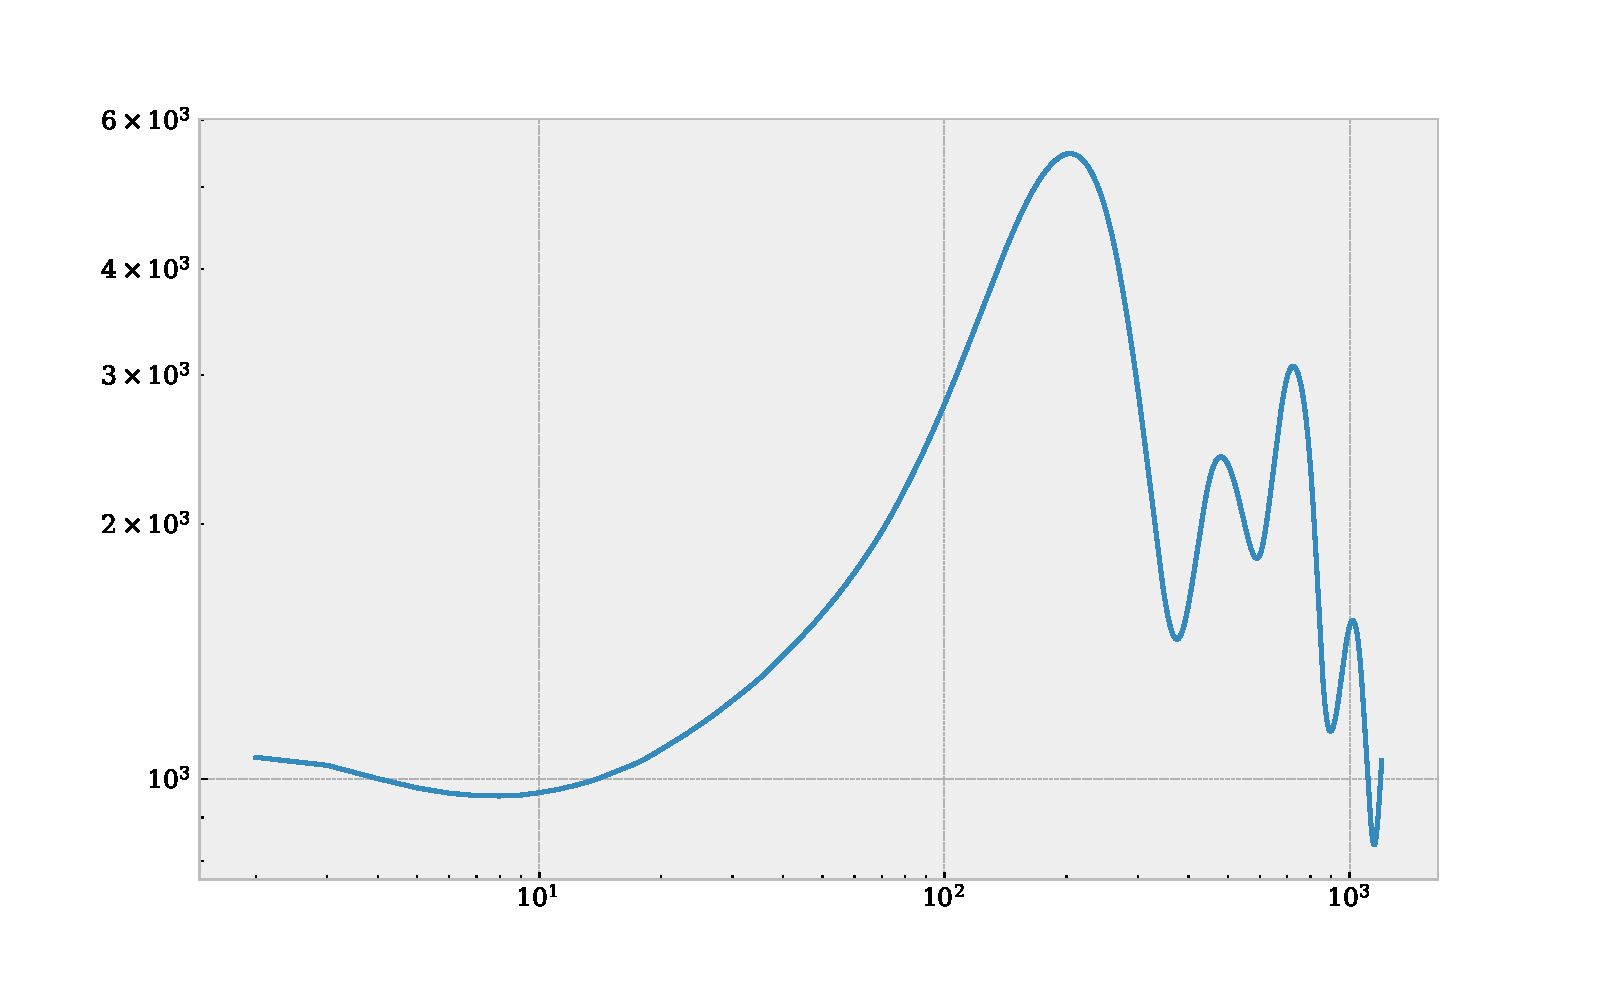
\includegraphics[scale = 0.65]{Figures/Cell.pdf}
    \caption{\textbf{Upper panel}: The figure shows the CMB angular power spectrum for different scales given by the multipole index $\ell$, for $0 < \ell < \ell_\text{max} = 1200$, in units $\mathrm{\mu K}^2$. The peaks and troughs are indicated as solid and dashed lines respectively. \textbf{Lower panel}: The figure shows the matter power spectrum as a function of the comoving wavenumber $k$. The scale $k_\text{eq} = 0.015 \mathrm{h / Mpc}$ of the horizon at matter-radiation equality is marked by a dashed red line.} 
    \label{fig:Cell}
\end{figure*}

\begin{figure*}
    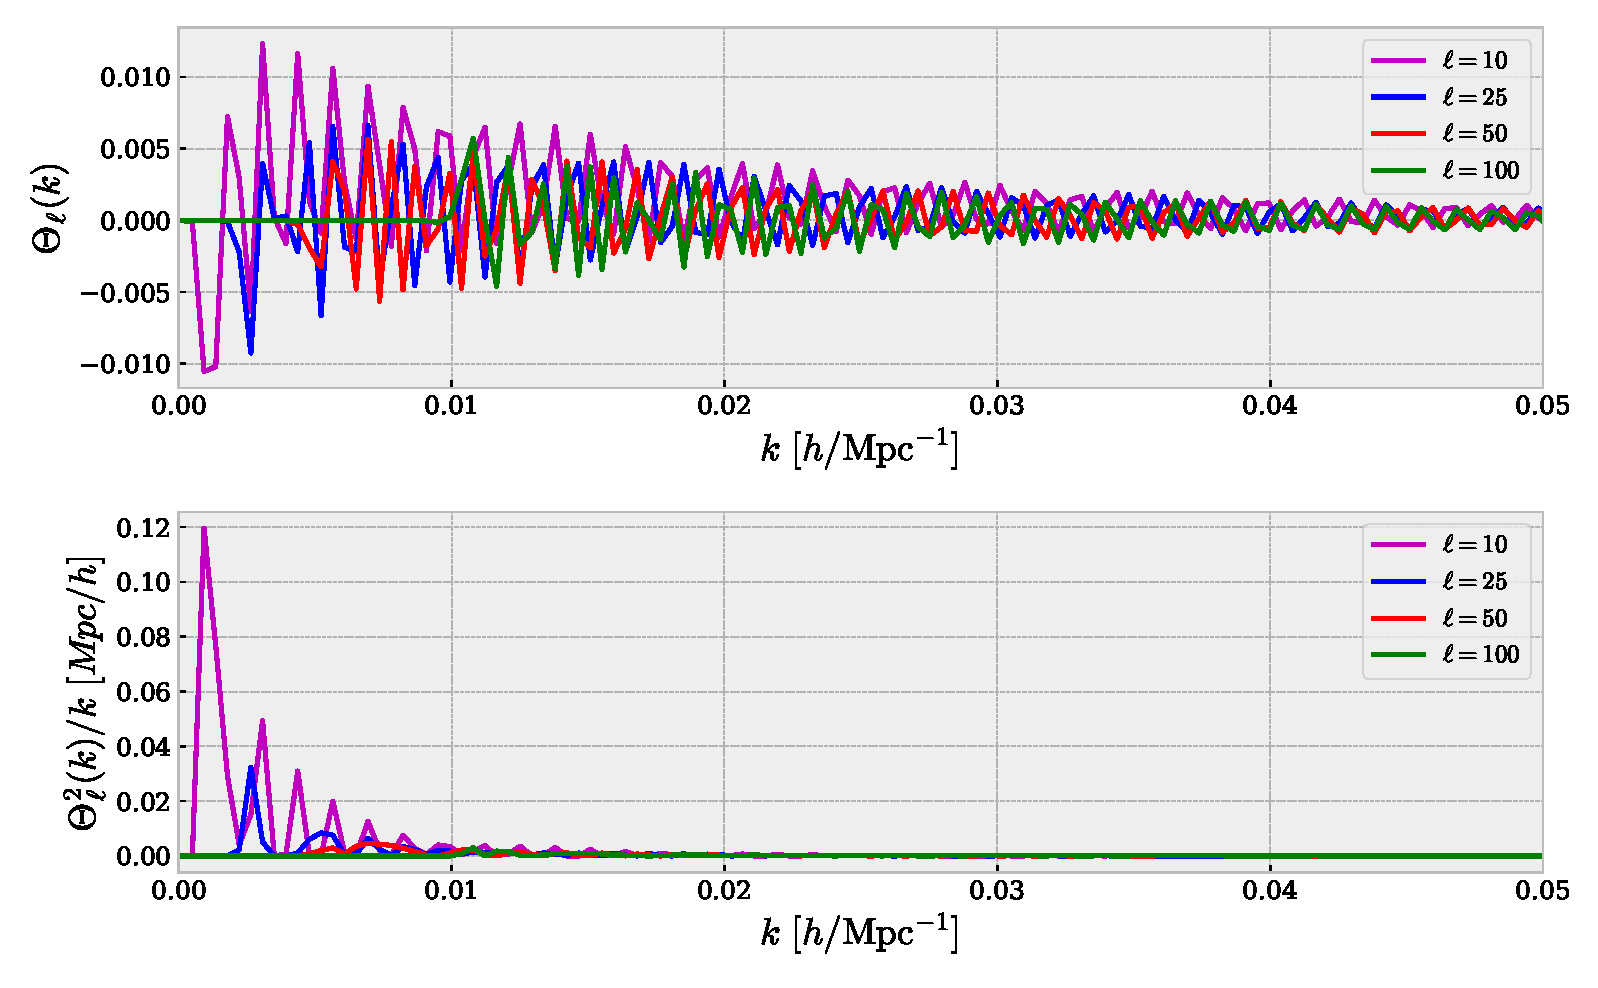
\includegraphics[scale = 0.65]{Figures/Transfer_func.pdf}
    \caption{\textbf{Upper panel}: The figure shows the radiation transfer functions $\Theta_\ell(k)$ as a function of comoving wavenumber $k$, for the multipoles $\ell = 10, 25, 50$ and $100$. \textbf{Lower panel}: The figure shows the integrand to the power spectrum (expept the primordial power spectrum bit) as a function of comoving wave number, for the multipoles $\ell = 10, 25, 50$ and $100$.}
    \label{fig:Transfer_func}
\end{figure*}

\section{Results / Discussion}\label{sec:Results/Discussion}

\section{Conclusion} \label{sec:Conclusion}

\newpage
\bibliography{ref}
\bibliographystyle{aasjournal}
\end{document}